% =====================================================================
% DSC 148 Final Report
%
% Predicting Team Success From Formation and Personnel in
% NCAA Division I Soccer
% =====================================================================

\documentclass[11pt,twocolumn]{article}

% --- Packages ----------------------------------------------------------
\usepackage[margin=0.85in,columnsep=0.25in]{geometry}
\usepackage{amsmath, amssymb}
\usepackage{graphicx}
\usepackage{booktabs}
\usepackage{caption}
\usepackage{subcaption}
\usepackage{float}
\usepackage{microtype}
\usepackage{hyperref}
\usepackage{xurl} % allow URLs to break anywhere (narrow two-column lines)
\usepackage[numbers,sort&compress]{natbib}
\usepackage{xcolor}
\usepackage{tabularx}
\usepackage{stfloats} % allow double-column floats at page bottom too

% Let wide (double-column) floats fill more of a page top/bottom so the
% result tables land on the Results page instead of cascading forward.
\renewcommand{\dbltopfraction}{0.92}
\renewcommand{\dblfloatpagefraction}{0.7}
\setcounter{dbltopnumber}{2}
\renewcommand{\textfraction}{0.05}

% Don't stretch inter-paragraph / inter-item glue to force full columns
% (avoids large gaps between bullets in two-column mode).
\raggedbottom

% Cleaner section spacing for a class report.
\usepackage{titlesec}
\titlespacing*{\section}{0pt}{1.2\baselineskip}{0.5\baselineskip}
\titlespacing*{\subsection}{0pt}{0.9\baselineskip}{0.3\baselineskip}

% Path prefix for figure includes (so we can compile from report/).
\graphicspath{{../artifacts/half_subs/_comparison_plots_v2/}{figures/}}

% --- Title block -------------------------------------------------------
\title{Predicting Team Success From Formation and Personnel in NCAA Division I Soccer}
\author{Zach Cochran \\
        \texttt{zcochran@ucsd.edu} \\
        DSC 148 --- Introduction to Data Mining \\
        University of California, San Diego}
\date{June 2026}

\begin{document}

% Full-width title + abstract spanning both columns.
\twocolumn[
  \begin{@twocolumnfalse}
  \maketitle
  \begin{abstract}
  \noindent
Predicting performance is a cornerstone of sports analytics, and in
soccer much of that performance comes down to tactics: which formation a
team plays and which players fill each role. We study whether these
choices can be predicted from data by modeling the expected goal (xG)
differential a team produces within a half. We compare several ways to
encode a lineup, including data-driven player archetypes, season
statistics, opponent information, and graph versus tabular
representations. Across sixteen model variants, a graph neural network
that combines data-driven archetypes with season statistics gave the
best result, predicting xG differential with an R$^2$ of $0.283$ and a
sign accuracy of $0.659$. These results suggest that team success can be
partially predicted from formation and personnel choices alone.
  \end{abstract}
  \vspace{1.5em}
  \end{@twocolumnfalse}
]

% =====================================================================
\section{Introduction}

\subsection{Problem and motivation}

Predicting success within a soccer match is difficult for several
reasons. In NCAA soccer, teams are allowed up to six substitution
windows per match, so the set of players on the pitch changes many times
within a match and within each half. To account for this, we model the
difference in xG within a half rather than across a full match. Modeling
at the half level lets the formation and personnel changes that happen at
halftime appear as separate rows in the dataset.

The aim of this prediction task is to learn whether certain play styles
across positions perform well together under given tactical conditions. A
model of this kind could be used to simulate how a team's expected
performance changes when a player switches positions, or whether a player
a team is recruiting fits tactically into the existing squad.

\subsection{Research questions}
Our goal is to determine whether specific tactical encoding choices help
predict success. We break this into four questions:

\begin{enumerate}
  \item \textbf{Personnel encoding.} Do data-driven player spatial
        archetypes beat raw position labels?
  \item \textbf{Quality encoding.} Does a player's season statistical
        profile improve prediction?
  \item \textbf{Opponent conditioning.} Does adding the opponent's
        lineup and personnel improve prediction (matchup vs.\ ego)?
  \item \textbf{Representation.} Does a graph neural network outperform a
        tabular XGBoost model?
\end{enumerate}

% =====================================================================
\section{Related Work}

\subsection{xG modeling}
Expected goals (xG) is the standard measure of shot quality in soccer.
Early models estimate the probability that a shot becomes a goal from
features such as shot location, body part, and defensive pressure, and
show that spatial and contextual features predict goals better than
distance alone~\citep{lucey2015}. Later models improve these estimates
using richer positional inputs and neural networks~\citep{anzer2021}.
These models work at the level of individual shots: each shot is scored
on its own, and a match's xG is the sum over its shots. Our task is
different. Instead of scoring shots, we predict the total xG differential
a team produces over part of a match from the players on the pitch and
how they are arranged, so the prediction reflects formation and personnel
rather than the shots that happened to be taken.

\subsection{Graph neural networks for soccer}
Graph neural networks suit team sports because the useful information
lies in how players relate to each other rather than in any single
player. In soccer, players are represented as nodes and tactical or
spatial relationships as edges, and message passing is used to predict
outcomes such as match results or the value of a play~\citep{xenopoulos2021}.
Many of these models use graph attention~\citep{velickovic2018} and the
PyTorch Geometric library~\citep{fey2019}. We build on this work but add
features specific to within-match tactics: edge types for substitutions
and for cross-team matchups based on shared time on the pitch, attention
over a fully connected within-team graph rather than a fixed proximity
graph, and node features that combine learned positional archetypes with
season statistics.

\subsection{Player role and archetype clustering}
Other work replaces fixed position labels with roles learned from data.
Bialkowski et al.\ learn team formations and player roles directly from
tracking data and find that the learned roles match tactical intuition
without supervision~\citep{bialkowski2014}. Related work describes
individual play style using feature spaces built from large public
event-data sets, so players can be compared by how
they play rather than by their listed position. We take the same
data-driven view but at a finer level: instead of one role per player, we
cluster event-level spatial tendencies within each position group to form
archetypes that describe different styles of playing the same position,
and we use these archetypes as node features in place of raw position
labels.

% =====================================================================
\section{Methods}

\subsection{Problem definition}
We treat each half of a match as one prediction example. For a half, let
team~$1$ and team~$2$ be the two teams, and let $\mathrm{xG}_1$ and
$\mathrm{xG}_2$ be the expected goals each team accumulates during that
half. These come from Wyscout's built-in xG values, summed over each
team's shots in the half. The target is the xG differential
\[
  y = \mathrm{xG}_1 - \mathrm{xG}_2 .
\]
The input is a snapshot of the half: the formation each team played, the
players who appeared and the minutes they were on the pitch, each
player's raw position and assigned archetype, and season-level statistics
for each player. A model takes this snapshot and predicts $\hat{y}$, an
estimate of the half's xG differential. A positive $y$ means team~$1$ was
expected to outscore team~$2$, so a model that recovers the sign of $y$
has identified which team was expected to do better.

\subsection{Data}
The data comes from Wyscout~\citep{pappalardo2019} and covers more than
$7{,}000$ NCAA Division I matches from 2020 to 2024. Each match has event
data, which records every on-ball event such as passes, shots, and duels,
and formation data, which records each team's lineup and formation.

We use the event data in two ways: to build the player archetypes used as
model features, and to aggregate event outcomes into season statistics
that are also used as features. The formation data is used to compute
minutes played for each player and to build the half snapshots from the
substitutions that occur during the match.

\subsection{Player archetypes}

\subsubsection{Position groups}
We first group Wyscout's raw position labels into eight categories:
center defenders (CD), left wide defenders (LWD), right wide defenders
(RWD), central midfielders (CM), center forwards (CF), left wide players
(LWP), right wide players (RWP), and goalkeepers (GK). These groups
capture the left/right and front/back asymmetry of player roles. Within
each group we then define styles of play, so that two players listed at
the same position can still play it in different ways.

\subsubsection{Intra-event clustering}
To define styles of play within a position group, we cluster each event
type separately. For example, for center defenders we form $12$ clusters
of passes using the pass start and end coordinates. Each cluster
corresponds to a common type of pass, and the share of a player's passes
that fall into each cluster describes part of their style. We repeat this
for every event type and position group, which gives a set of clusters
that any player's events can be grouped into. Figure~\ref{fig:intra-event-cd}
shows the clusters for center defenders.

\begin{figure}[H]
\centering
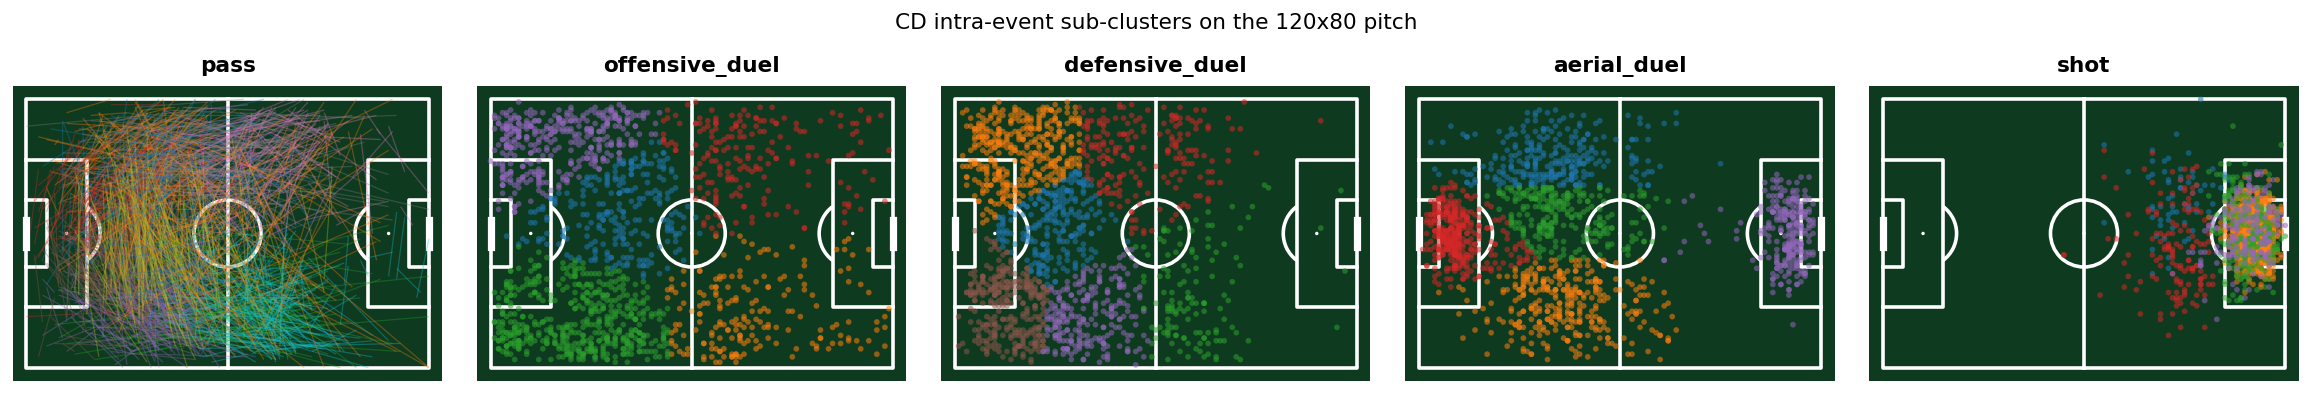
\includegraphics[width=\linewidth]{intra_event_cd.png}
\caption{Intra-event $k$-means sub-clusters for center defenders. Each
panel is one center-defender event type, with points colored by cluster.
(All-groups version: Appendix~\ref{app:intra-event-all}.)}
\label{fig:intra-event-cd}
\end{figure}

\subsubsection{Player-season aggregation}
We then aggregate, for each player and season, the events that fall into
each cluster. From these counts we build a vector that represents the
player's spatial tendencies: the proportion of each event type they
perform, and how those events are distributed across the clusters.

\subsubsection{Archetype clustering}
Finally, we run $k$-means on the player-season spatial vectors to group
players with similar tendencies into archetypes, separately for each
position group. These archetypes are the features used by the models.
Figure~\ref{fig:archetype-bars-cd} shows the center-defender archetypes
and how their spatial tendencies differ.

\begin{figure}[H]
\centering
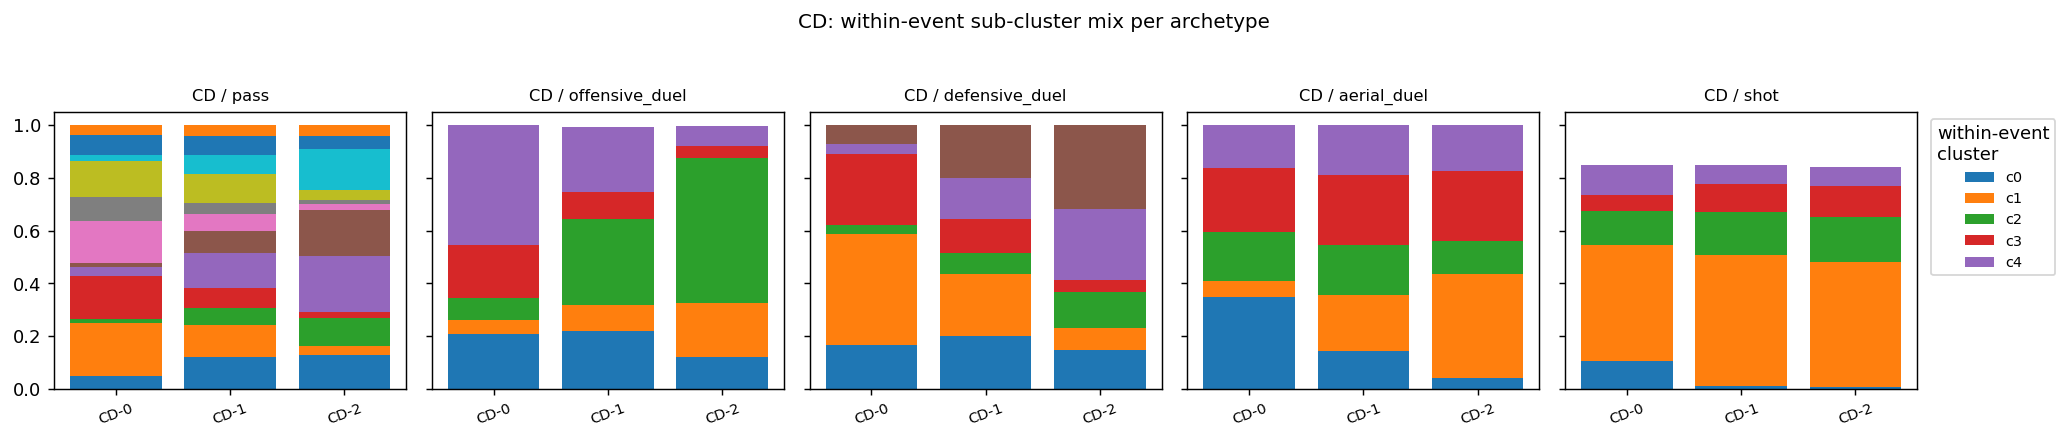
\includegraphics[width=\linewidth]{archetype_bars_cd.png}
\caption{Within-event sub-cluster mix per archetype for center
defenders. Each panel is one event type; stacked bars give the mean
proportion of each archetype's events that fall into each within-event
sub-cluster. (All-groups version: Appendix~\ref{app:archetype-bars-all}.)}
\label{fig:archetype-bars-cd}
\end{figure}

\subsection{Dataset construction}
We build one snapshot per half. A snapshot records the formation a team
played, every player who appeared in the half with the minute they
entered and left the pitch, and each player's archetype and raw position.
We also attach each player's season statistics. The target is the xG
differential between the two teams in that half.

We split the data $80/20$ into train and test sets, blocked by match so
that both halves of a match fall in the same split. Every model variant
is trained on the same training set and evaluated on the same held-out
test set, so the results are directly comparable.

\subsection{Models}

\subsubsection{Tabular XGBoost baseline}
The baseline is a gradient-boosted tree model~\citep{chen2016} trained on
the dataset in its tabular form. It learns the relationship between the
lineup features and the target without any explicit graph structure.

\subsubsection{Graph neural network}
The graph model takes the lineup for each half and builds a graph from
it. A graph matches how soccer lineups are normally structured, drawn,
and reasoned about: players are nodes and the relationships between them
are edges, which lets the model represent how players interact and
contribute to the team. The architecture is as follows:
\begin{itemize}
  \item \textbf{Node set.} Variable: the $11$ starters plus any
        substitutes who appeared in the half (typically $3$--$6$).
        Players are placed in a hand-crafted template based on the
        team's formation, matching how lineups are usually drawn.
  \item \textbf{Node features.} Position encoding (raw position or
        archetype), season statistics, minutes played, and position
        within the formation template.
  \item \textbf{Edge types.}
        \begin{enumerate}
          \item \emph{Intra-team}: relationships between teammates.
          \item \emph{Sub}: substitution information.
          \item \emph{Matchup}: how a player relates to an opposing
                player.
        \end{enumerate}
  \item \textbf{Edge features.} A same-team flag, the relative distance
        between positions in the formation, and, for matchup edges, the
        differences in player statistics (for example, a strong winger
        against a weak defender).
\end{itemize}
Figure~\ref{fig:graph-modes} shows both graph construction modes.

\begin{figure}[H]
\centering
\begin{subfigure}{\linewidth}
  \centering
  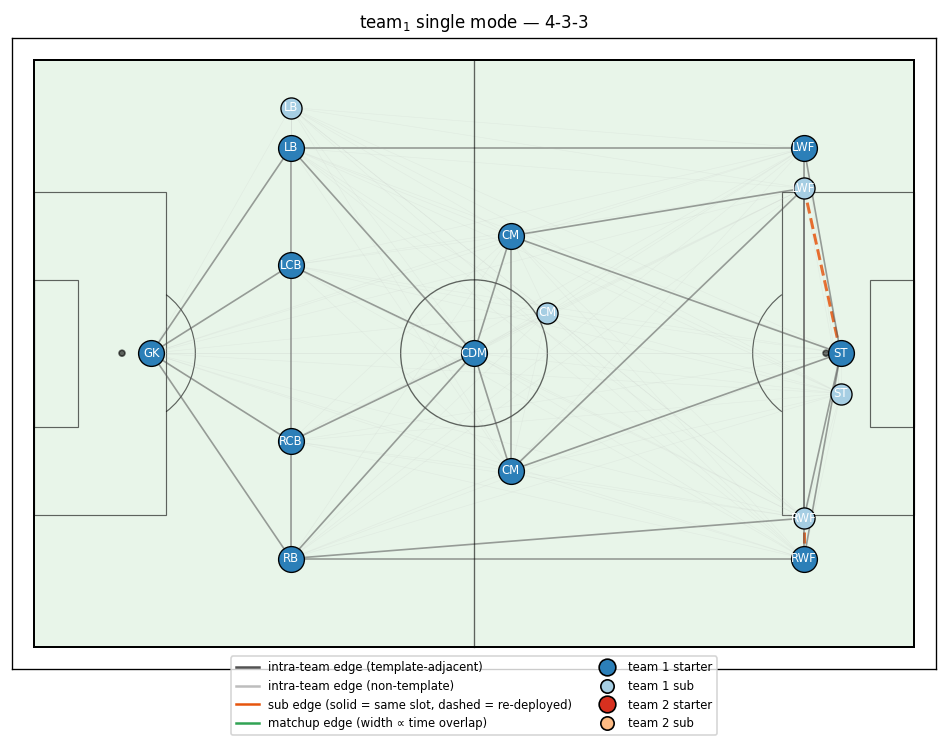
\includegraphics[width=\linewidth]{graph_single_team1.png}
  \caption{\textbf{Single mode.} Team$_1$'s self-contained subgraph
  (a $4{-}3{-}3$).}
  \label{fig:graph-single}
\end{subfigure}

\vspace{0.8em}

\begin{subfigure}{\linewidth}
  \centering
  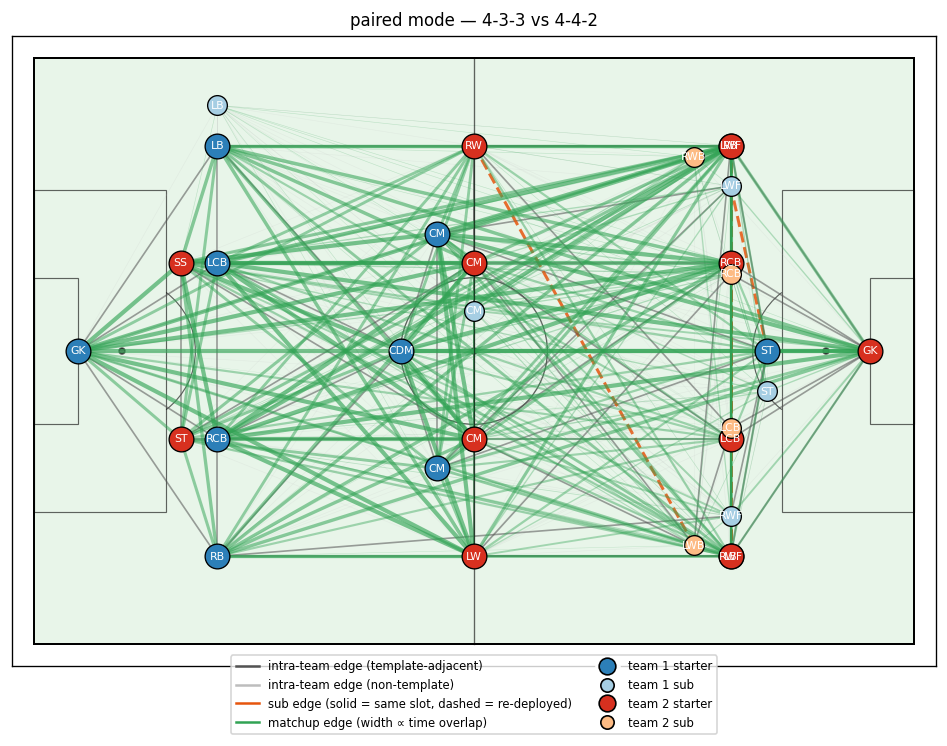
\includegraphics[width=\linewidth]{graph_paired.png}
  \caption{\textbf{Paired mode.} Both teams in one $22+$-node graph.}
  \label{fig:graph-paired}
\end{subfigure}
\label{fig:graph-modes}
\end{figure}

\subsubsection{Model variants}
Each model family has $2{\times}2{\times}2$ variants along three axes of
tactical encoding:
\begin{itemize}
  \item \textbf{Personnel encoding.} \texttt{position} (raw position
        labels) vs.\ \texttt{archetype} (data-driven clusters).
  \item \textbf{Opponent conditioning.} \texttt{ego} (single-team graph)
        vs.\ \texttt{matchup} (paired-team graph).
  \item \textbf{Quality encoding.} \texttt{no\_stats} (no season stats)
        vs.\ \texttt{stats} (10-D player-season stats, plus stat-diff
        matchup features).
\end{itemize}

% Tables contributed just before the section so the double-column floats
% can claim the top of the Results page rather than cascading forward.
\begin{table*}[t]
\centering
\label{tab:full-grid}
\resizebox{\textwidth}{!}{\small
\begin{tabular}{llllrrrrr}
\toprule
kind & opponent & stats & family & MAE & RMSE & MSE & R$^2$ & sign acc \\
\midrule
arch & ego & no & gnn & 0.3415 & 0.4611 & 0.2126 & 0.1848 & 0.6174 \\
arch & ego & no & tab & 0.3673 & 0.4982 & 0.2482 & 0.0483 & 0.5838 \\
arch & ego & yes & gnn & 0.3217 & 0.4362 & 0.1902 & 0.2706 & 0.6519 \\
arch & ego & yes & tab & 0.3538 & 0.4793 & 0.2298 & 0.1191 & 0.5973 \\
arch & matchup & no & gnn & 0.3419 & 0.4640 & 0.2153 & 0.1744 & 0.6067 \\
arch & matchup & no & tab & 0.3446 & 0.4689 & 0.2198 & 0.1572 & 0.6151 \\
arch & matchup & yes & gnn & \textbf{0.3202} & \textbf{0.4326} & \textbf{0.1871} & \textbf{0.2826} & \textbf{0.6592} \\
arch & matchup & yes & tab & 0.3246 & 0.4415 & 0.1949 & 0.2526 & 0.6467 \\
pos & ego & no & gnn & 0.3623 & 0.5034 & 0.2534 & 0.0285 & 0.5459 \\
pos & ego & no & tab & 0.3918 & 0.5275 & 0.2782 & -0.0668 & 0.5397 \\
pos & ego & yes & gnn & 0.3276 & 0.4437 & 0.1969 & 0.2450 & 0.6352 \\
pos & ego & yes & tab & 0.3507 & 0.4733 & 0.2240 & 0.1410 & 0.6028 \\
pos & matchup & no & gnn & 0.3648 & 0.5073 & 0.2574 & 0.0132 & 0.5326 \\
pos & matchup & no & tab & 0.3938 & 0.5246 & 0.2752 & -0.0552 & 0.5825 \\
pos & matchup & yes & gnn & 0.3269 & 0.4431 & 0.1963 & 0.2473 & 0.6498 \\
pos & matchup & yes & tab & 0.3274 & 0.4407 & 0.1942 & 0.2555 & 0.6433 \\
\bottomrule
\end{tabular}
}
\end{table*}

\begin{table*}[t]
\label{tab:ablation-summary}
\centering
\begin{tabular}{lrrrrr}
\toprule
Design axis & MAE & RMSE & MSE & R$^2$ & sign acc \\
\midrule
archetype - position & -0.0162 & -0.0227 & -0.0222 & +0.0851 & +0.0308 \\
stats - no-stats & -0.0319 & -0.0456 & -0.0433 & +0.1662 & +0.0578 \\
matchup - single & -0.0091 & -0.0125 & -0.0116 & +0.0446 & +0.0202 \\
gnn - XGBoost & -0.0184 & -0.0203 & -0.0194 & +0.0744 & +0.0110 \\
\bottomrule
\end{tabular}
\end{table*}


% =====================================================================
\section{Results}
\subsection{Model performance}

The best model reaches an R$^2$ of $0.283$ and a sign accuracy of
$0.659$, meaning it explains about $28\%$ of the variance in xG
differential and correctly calls which team was expected to outperform
the other in roughly $66\%$ of halves. This model uses every tactical
encoding we tested: data-driven archetypes, the matchup graph, and season
statistics. The encodings stack, with each one adding to predictive
performance rather than replacing another.

Season statistics matter most. Adding them raises R$^2$ by $0.166$ and
lowers MSE by $0.043$, far more than any other encoding. Season
statistics capture the difference in player quality across lineups, which
is a large part of what decides a half. They are also the easiest
encoding to add, since they only require aggregated season totals and no
event data. That makes them a practical option for analysts who want a
similar model but cannot build data-driven archetypes.

The archetypes also help, raising R$^2$ by $0.085$ and lowering MSE by
$0.022$. Knowing how a player tends to play their position, not just
which position they play, improves the prediction, and the model can use
the mix of archetypes in a lineup. Archetypes cost more to build than
season statistics because they need event data, but they add a clear gain
on top of the statistics.

How the lineup is represented also matters. The graph form lets the model
use the structure of the lineup and the relationships between players
directly. The GNN raises R$^2$ by $0.074$ and lowers MSE by $0.019$ over
the tabular baseline, so the graph captures lineup information that the
tabular model misses.

The opponent conditioning helps least, raising R$^2$ by only $0.045$ and
lowering MSE by $0.011$. Most of a team's expected output seems to come
from its own tactics and player quality rather than the specific
opponent. Opponent information is not useless, but it appears to add value
mainly once a team's own choices are accounted for, so teams are better
off optimizing their own lineup before tailoring it to an opponent.

\subsection{Limitations}

A major limitation is that college soccer allows many substitutions,
which adds noise to the lineup even within a half and makes it harder for
the model to learn the relationship between the lineup and the xG
differential. The model may perform better in professional leagues, where
there are fewer substitutions and more tactical consistency within a
match.

A second limitation is that the data spans every conference in Division I,
where team and player quality vary widely. This variation adds noise.
Normalizing player statistics across conferences could reduce it and let
the model focus on the tactical relationships rather than raw quality
differences.

A third limitation is the absence of match-level features such as home or
away and travel distance. Home advantage is real in college soccer, and
pitch type (grass versus turf) and weather vary across matches; teams
unused to certain conditions may underperform. College athletes are also
students, so heavy travel for away games can cause fatigue and less
preparation time, which professional teams do not face to the same
degree. None of this is currently captured.

A final limitation is that the archetypes require event data, which not
every analyst can access. Our results show that season statistics alone
already give useful predictions, but the archetypes add a clear gain on
top of them, so there is value in building archetypes where event data is
available.

\subsection{Future work}

One main use of this model is to simulate how different players would
perform in a team's current lineup. This would let us estimate how a new
signing or a position change would affect expected performance, which
could help coaches and analysts make recruitment and selection decisions.

A second direction is to learn the archetypes end-to-end inside the xG
model rather than building them separately. Letting the model learn the
spatial tendencies most useful for predicting xG differential could
improve performance further.

A third direction is to apply the model to professional leagues, where
there are fewer substitutions and more tactical consistency. This would
test whether the same encodings work in a different setting, and whether
the importance of each encoding changes across leagues.

% =====================================================================
\section{Conclusion}

This study looks at predicting team success from tactical lineup
encodings, a task that matters for selecting game-day rosters and
recruiting players. We encoded formations and personnel in several ways
and described a data-driven method for building player spatial archetypes
within position groups, which separates players by how they play their
position. We then used graph neural networks to learn which styles of play
work well together. The best model, a graph neural network using
archetypes, player statistics, and opponent conditioning, predicted xG
differential with an R$^2$ of $0.283$. The approach is a promising
starting point for predicting team success from formation and personnel.

% =====================================================================
\section*{Data and Code Availability}
The match and event data are from Wyscout. The
code used to build the archetypes, construct the dataset, and train and
evaluate the models is available from the author at
\url{https://github.com/zcochran27/team-success-prediction-via-formation-and-personnel}.

% =====================================================================
% Bibliography
\bibliographystyle{plainnat}
\begin{thebibliography}{10}

\bibitem{lucey2015}
P.~Lucey, A.~Bialkowski, M.~Monfort, P.~Carr, and I.~Matthews.
``Quality vs.\ Quantity: Improved Shot Prediction in Soccer using
Strategic Features from Spatiotemporal Data.''
\emph{MIT Sloan Sports Analytics Conference}, 2015.

\bibitem{anzer2021}
G.~Anzer and P.~Bauer.
``A Goal Scoring Probability Model for Shots Based on Synchronized
Positional and Event Data in Football (Soccer).''
\emph{Frontiers in Sports and Active Living}, 3:624475, 2021.

\bibitem{xenopoulos2021}
P.~Xenopoulos and C.~Silva.
``Graph Neural Networks to Predict Sports Outcomes.''
\emph{IEEE International Conference on Big Data (Big Data)}, 2021.

\bibitem{velickovic2018}
P.~Veli\v{c}kovi\'c, G.~Cucurull, A.~Casanova, A.~Romero, P.~Li\`o, and
Y.~Bengio.
``Graph Attention Networks.''
\emph{International Conference on Learning Representations (ICLR)}, 2018.

\bibitem{fey2019}
M.~Fey and J.~E.~Lenssen.
``Fast Graph Representation Learning with PyTorch Geometric.''
\emph{ICLR Workshop on Representation Learning on Graphs and Manifolds},
2019.

\bibitem{bialkowski2014}
A.~Bialkowski, P.~Lucey, P.~Carr, Y.~Yue, S.~Sridharan, and I.~Matthews.
``Identifying Team Style in Soccer using Formations Learned from
Spatiotemporal Tracking Data.''
\emph{IEEE International Conference on Data Mining Workshops (ICDMW)},
2014.

\end{thebibliography}

% =====================================================================
\appendix
\onecolumn % appendix grids are full-page; render them single-column
\section{Intra-event sub-clusters, all position groups}
\label{app:intra-event-all}
The all-groups version of Figure~\ref{fig:intra-event-cd}: each row is
one position group, each column is an event type. Where a group has
fewer event types than the maximum, trailing panels are blank. The
$k$-selection summary (elbow + silhouette per pair) is in the
\texttt{event\_clustering} notebook outputs.

\begin{figure}[H]
\centering
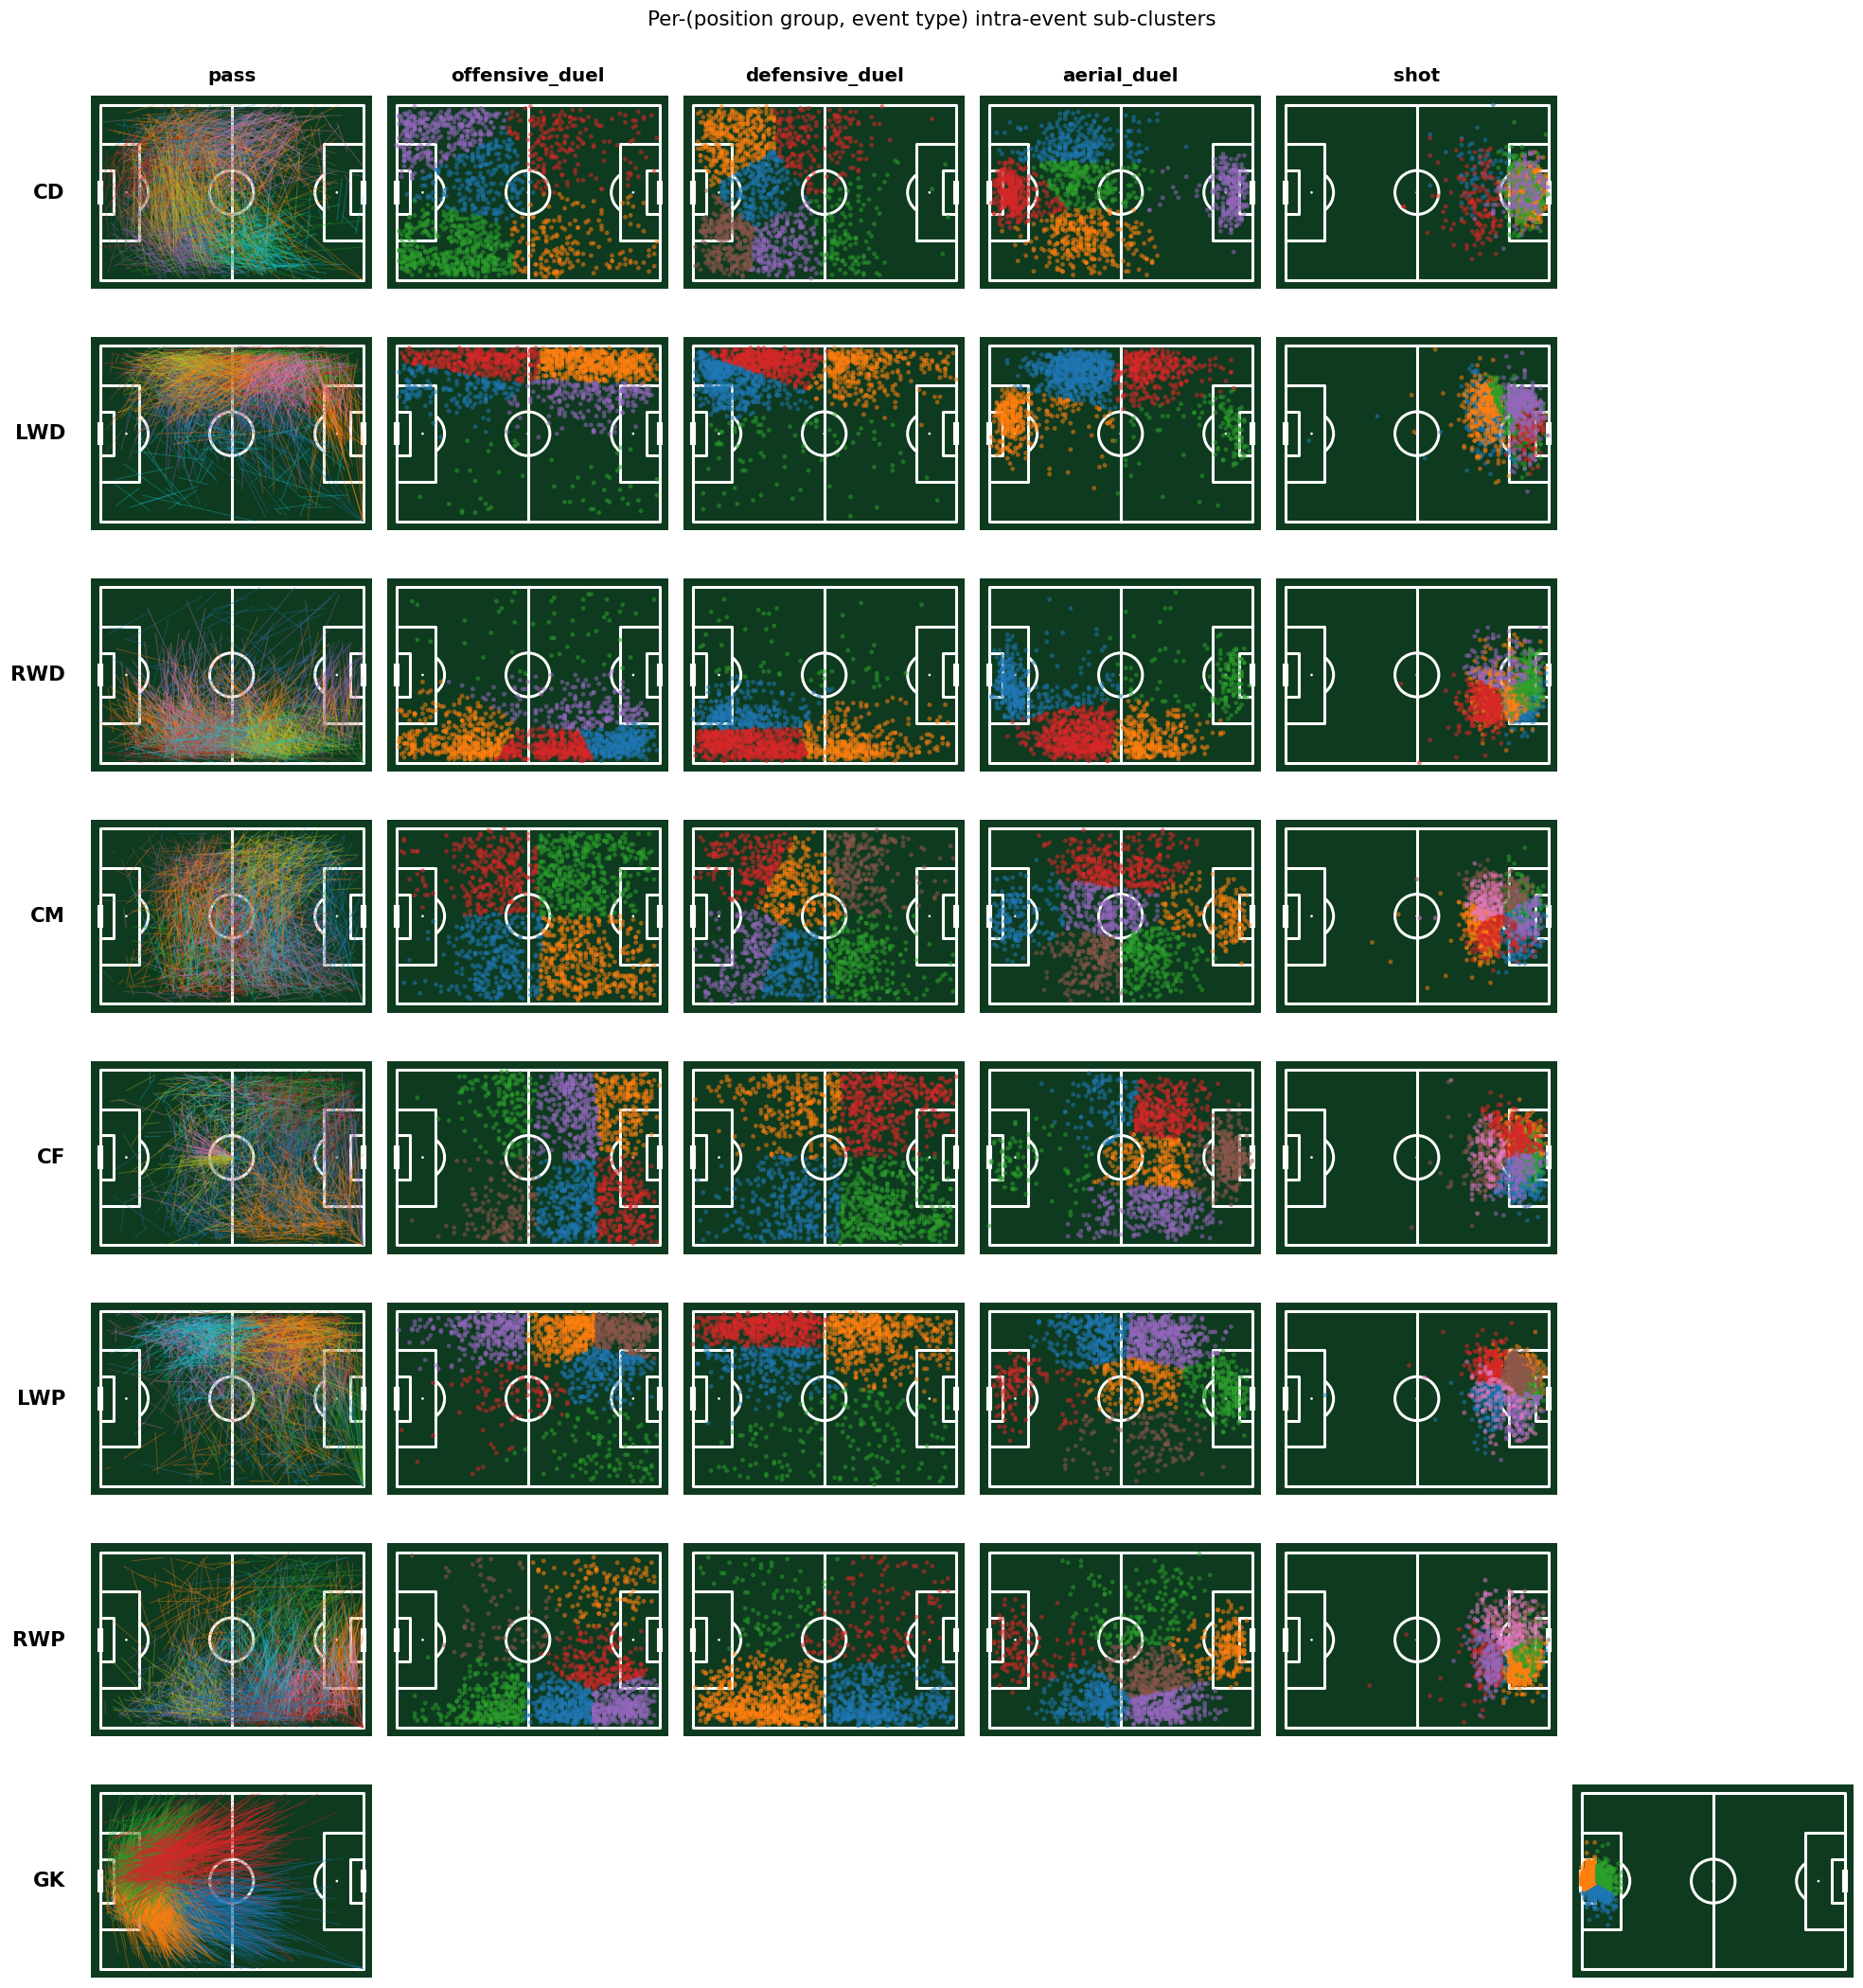
\includegraphics[width=\linewidth]{intra_event_all_groups.png}
\caption{Intra-event sub-clusters for every (position group, event
type) pair. Compare any single row against Figure~\ref{fig:intra-event-cd}
(the CD row).}
\label{fig:intra-event-all-appendix}
\end{figure}

\section{Within-event sub-cluster mix per archetype, all groups}
\label{app:archetype-bars-all}
The all-groups version of Figure~\ref{fig:archetype-bars-cd}: each row
is one position group, each column is an event type, stacked bars give
the proportional sub-cluster mix of that group's archetypes.

\begin{figure}[H]
\centering
% Cap the height so the heading + grid share one page (no blank-space gap).
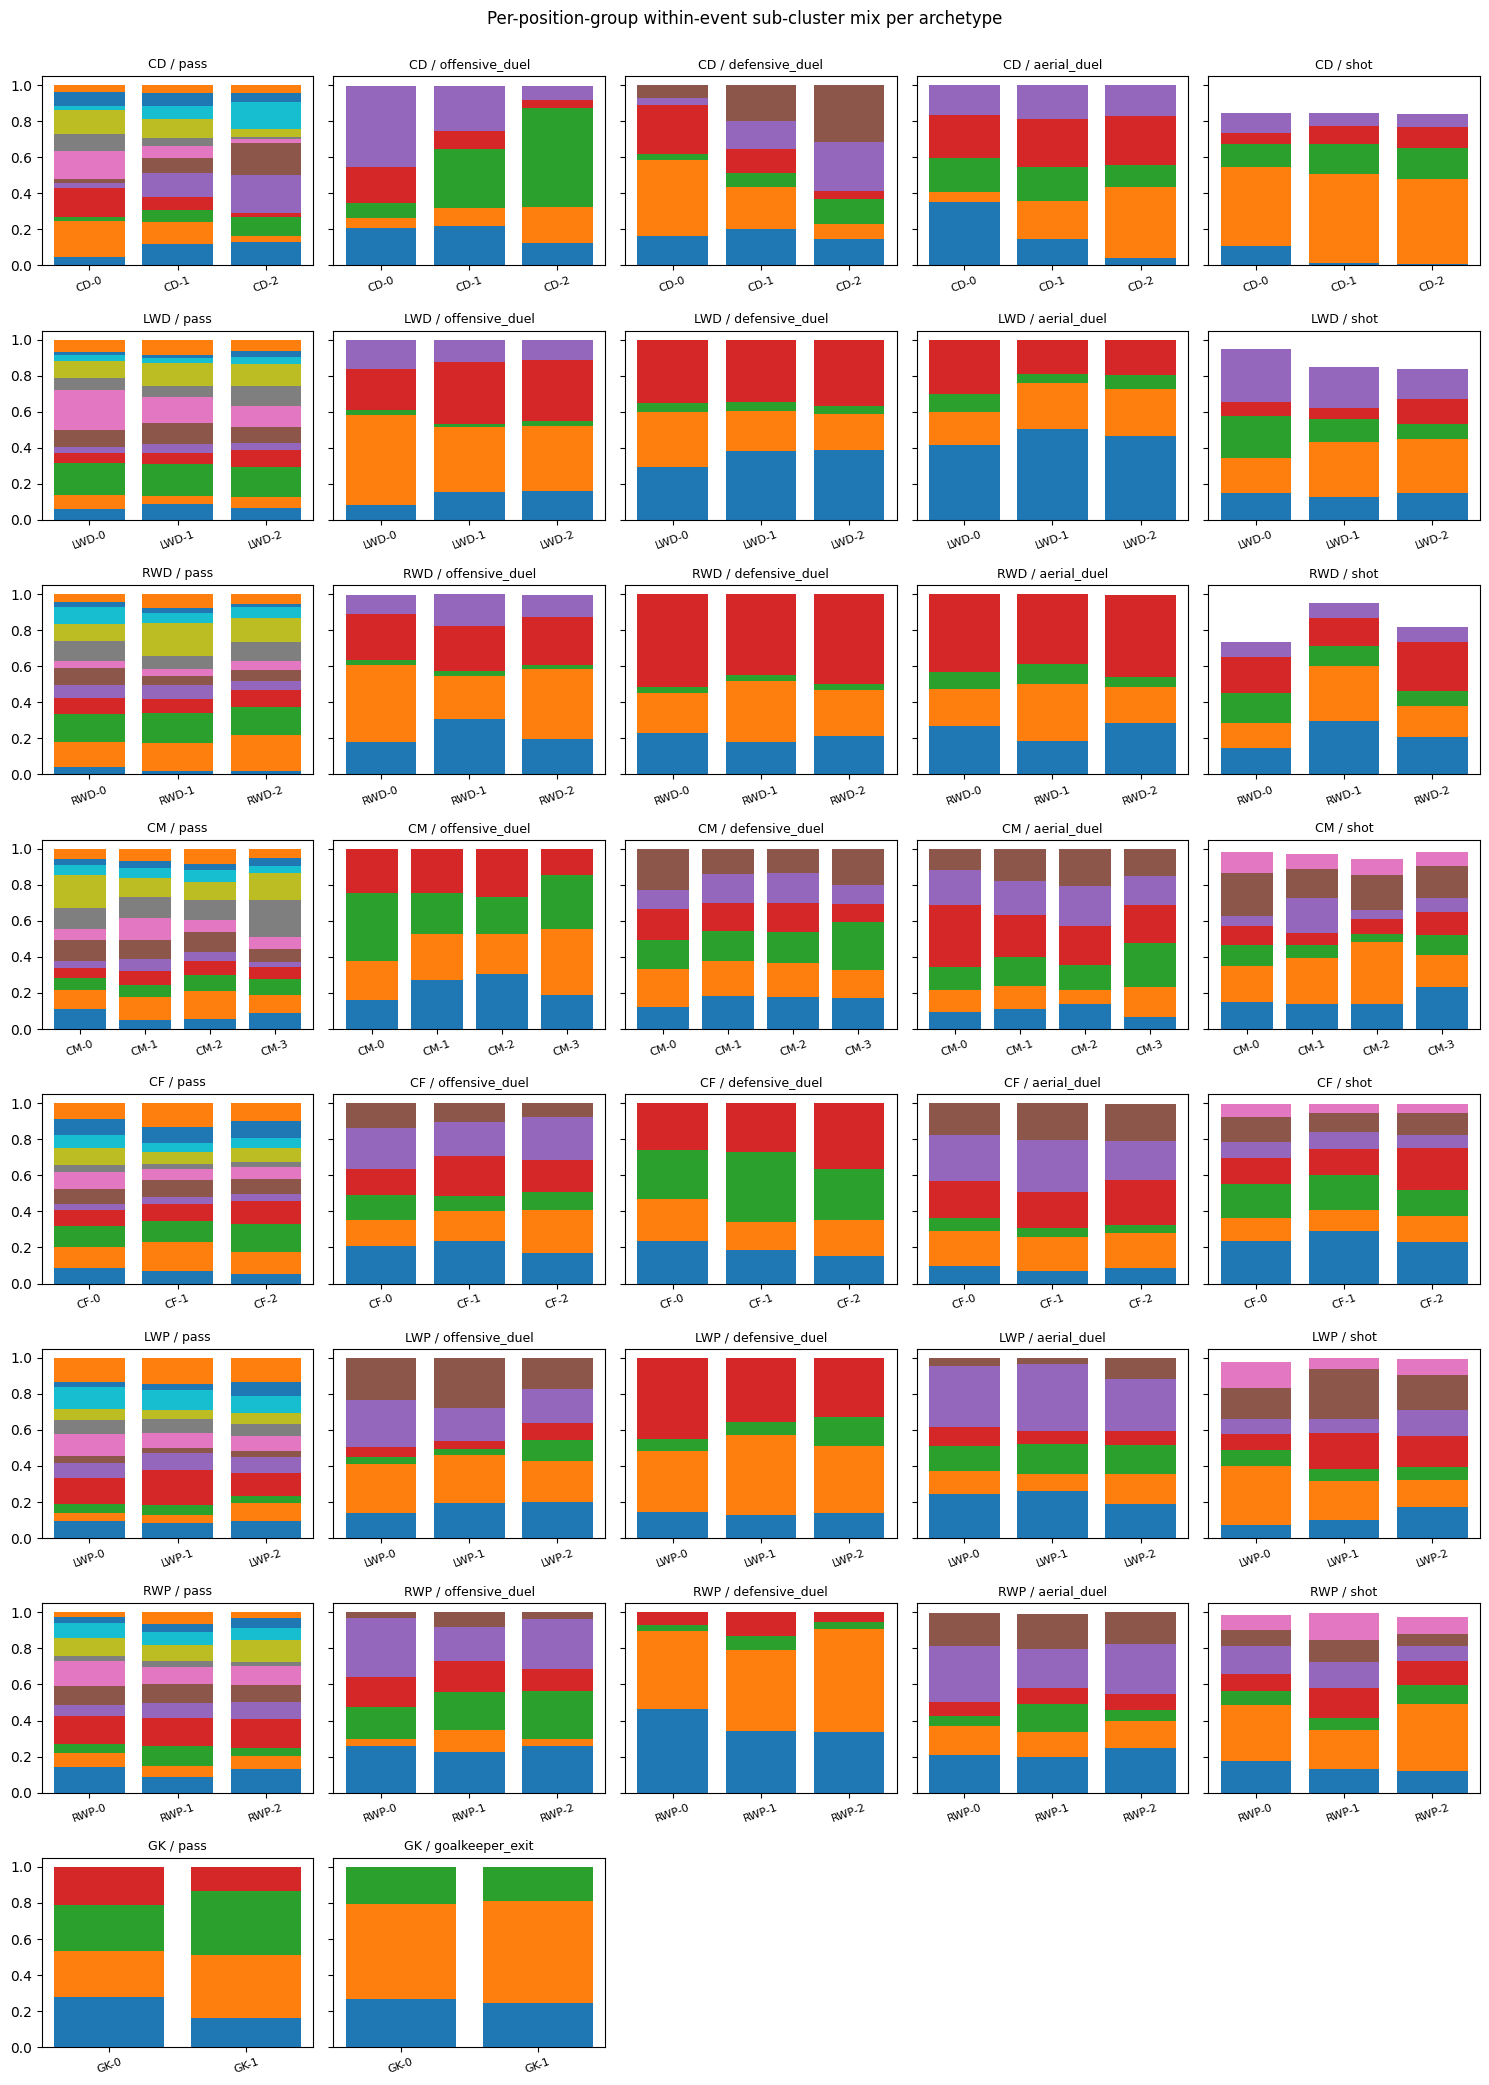
\includegraphics[width=\linewidth,height=0.82\textheight,keepaspectratio]{archetype_bars_all_groups.png}
\caption{Within-event sub-cluster mix per archetype, every position
group. Compare any single row against Figure~\ref{fig:archetype-bars-cd}
(the CD row).}
\label{fig:archetype-bars-all-appendix}
\end{figure}

\end{document}
